\documentclass[11pt]{beamer}
\usetheme{Singapore}

\usepackage[utf8]{inputenc}
\usepackage[T1]{fontenc}
\usepackage{soul}
\usepackage{graphicx}


\graphicspath{{../Figures/}}

\def\et{{\it et al.}}


\author{Cody Glickman \\ CPBS Update Talk}

\title{Hodgepodge Metagenomics: \\ A collection of novel tools for viral and bacterial sequences}
%\subtitle{}
%\logo{}

\date{ 
\includegraphics[height=2cm, width=2cm]{lablogo.png} \\ Jan 29th, 2018}
%\subject{}
\setbeamercovered{transparent}
\setbeamertemplate{navigation symbols}{}
\setbeamertemplate{theorems}[numbered]

\begin{document}
	\maketitle
	\begin{frame}{Table of Contents}
		\tableofcontents
		%\column{0.4\textwidth}
		%\includegraphics[height=5.5cm, width=5cm]{kaola.png}
		%\end{columns}
	\end{frame}
	
	
\section{Introduction}
\subsection{}

	\begin{frame}{Non-Tuberculosis Mycobacterial (NTM) Infections}
	
		\begin{block}{Number of Cases}
		The number of NTM cases is estimated over 100K
		\end{block}
		
		\begin{block}{Increasing Case}
		The rate of cases is estimated to grow at 8\% every year
		\end{block}
		
		
		\begin{block}{Populations at risk of developing NTM}
		\begin{itemize}
		\item Immunocompromised individuals 
		\item Patients with lung damage or malfunction 
		\item Residing in warm costal areas especially Hawaii
		\end{itemize}
		\end{block} 
		
		\begin{block}
		
		\end{block}
		
	\tiny{Strollo SE, et al. Ann Am Thorac Soc. 2015 \\
	Adjemian J, et al. Am J Respir Crit Care Med. 2012}
	
	\end{frame}
	
	\begin{frame}{Connecting NTM to Metagenomics}
	
	\begin{block}{The curious case of NTM}
	\begin{itemize}
	\item Certain populations 
	\item Lady Windemere Syndrome
	\end{itemize}
	\end{block}
	
	\begin{block}{Location, Location, Location}
	Why do NTM infections so commonly occur in the lung? 
	\end{block}
	
	
	
	
	\end{frame}
	
	
	\begin{frame}{Of "Viral" Importance}
	\begin{columns}
	\column{0.7\textwidth}
	
	\begin{block}{Bacteriophages aka Phages}
	Phages are DNA viruses that infect prokaryotes
	\end{block}
	
	\begin{block}{Bacteriophage Adherence to Mucus (BAM)}
	\begin{itemize}
	\item \alert{Phages act as an innate immune system in mucosal tissues}
	\item Prior studies identified Ig-like motifs in induced phages from Pseudomonas cultures
	\end{itemize}
	\end{block}
	
	\begin{block}{Phages in the Lungs}
	The abundance of phages is significantly lower in the lungs
	\end{block}
	
	\column{0.4\textwidth}
	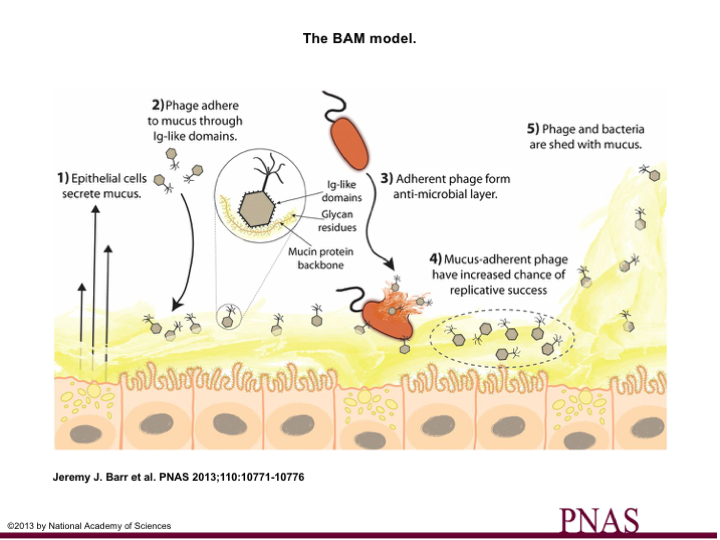
\includegraphics[height=5.5cm, width=5cm]{barr.png}
	\end{columns}

	
	
	
	\end{frame}
	
	
	\begin{frame}{Molecular Methods to Study Phages}
	\begin{columns}
	\column{0.6\textwidth}
	\begin{block}{Difficulties of phage study}
	\begin{itemize}
		\item Lack of universal marker gene
		\item Sequence heterogeneaity 
		\item Misclassification in databases
	\end{itemize}
	\end{block}
		
		
	\begin{block}{Phage Isolation Methods}
	\begin{itemize}
		\item Biological filtration
		\item In Silico Methods
	\end{itemize}
	\end{block}
	
	\column{0.4\textwidth}
		%%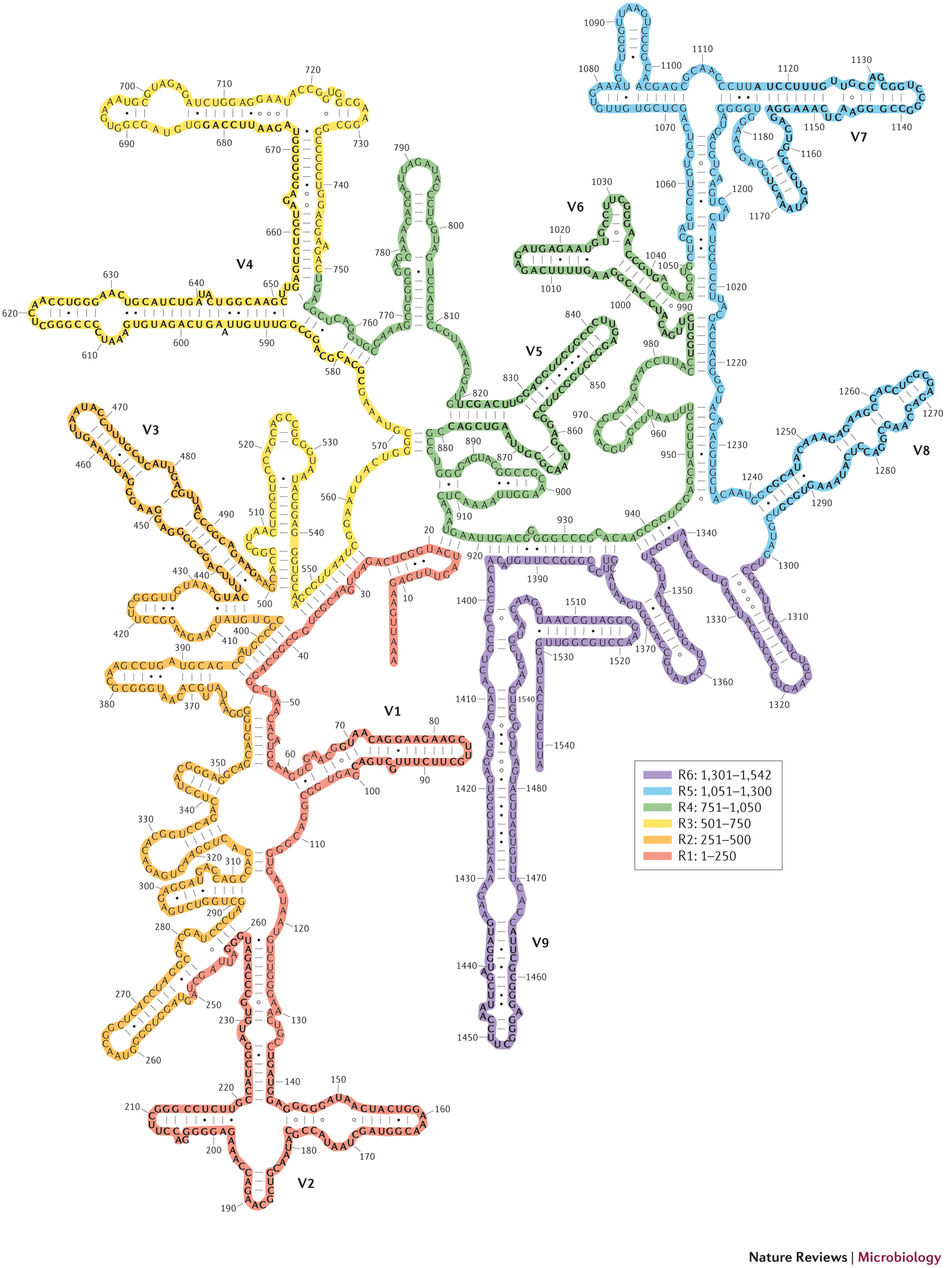
\includegraphics[height=5.5cm, width=5cm]{ribosome.png}
	\end{columns}
		
	
	\end{frame}

	
	\begin{frame}{Objective}
	
	Develop new tools and incorporate them into pipelines to identify and quantify bacteriophage elements in shotgun metagenomic sequences.
	
	\begin{block}{Secondary Goal}
	Identify relationships between bacteria and phages using the quantification across multiple studies. 
	\end{block}
	\end{frame}
	
\section{Metagenomic Simulation Study}
\subsection{}
	
	\begin{frame}{Metagenomics Gold Standard}
	CAMI
	%% ADD More HERE!!
	Why Viruses cause worsening performance?
	Why the gold standard was Pyrete
	\end{frame}
	
	\begin{frame}{Viral Metagenomics Gold Standard} 
	
	
	\end{frame}
	
	\begin{frame}{Study Design}
	\hyperlink{https://github.com/glickmac/Novel_Viral_Discovery}{This study establishes the feasibility for the filtration and novel viral identification pipeline in development.}
	
	\begin{block}{Simulation Study}
	A simulated mixed metagenome is used to compare the viral taxonomic identification performance
	\end{block}
	
	\begin{block}{Sensitivity Study}
	A real longitudinal metagenomic dataset is spiked with a rare virus to measure sensitivity of taxonomic assignments. 
	\end{block}
	
	\end{frame}
	
	
	\begin{frame}{Tools Used in Study}
	The tools used in this study are selected based on recent publications
	\begin{block}{Assembler}
	MEGAHIT - Effective at assembling viromes \\
	\tiny{Roux, Simon, et al. PeerJ 2017}
	\end{block}
	
	\begin{block}{Filtration Methods}
	VirFinder - Viral contig K-mer identification model \\ 
	\tiny{Ren, Jie, et al. Microbiome 2017}
	
	\large{Blastx - Filtering against a viral protein database} \\
	\tiny{Camacho C., et al. BMC Bioinformatics 2008}
	\end{block}
	
	\end{frame}
	
	\begin{frame}{Tools Used in Study Continued}
	\begin{block}{Simulation Tools}
	BBMAP - a suite of tools designed for sequencing data \\
	\tiny{Bushnell, B., JGI 2016}
	\end{block}
	
	\begin{block}{Taxonomic Identification}
	Kraken - A reference-free K-mer taxonomic identifier \\
	\tiny{Wood, Derrick E., and Steven L. Salzberg Genome 2014}
	
	\large{Blastx - Referenced against a viral protein database} \\
	\tiny{Camacho C., et al. BMC Bioinformatics 2008}
	\end{block}
	
	\begin{block}{Prophage Identification}
	Phaster - A popular prophage discovery web tool  \\
	\tiny{Arndt, David, et al., Nucleic Acids Research 2016}
	\end{block}
	\end{frame}
	
	
\section{GRAB}
\subsection{}
	
	\begin{frame}{Genomes in Simulation}
	\begin{columns}
		\column{.5\textwidth}
			\begin{block}{Virus - 0.12 Mb}
			\begin{itemize}
			\item Bacillus phage Pony
			\item Caulobacter phage CcrColossus
			\item Mycobacterium phage Bxb1
			\item Mycobacterium phage Che9d
			\item Mycobacterium phage TM4
			\item Pseudomonas phage vB-PaeM-C2-10-Ab1
			\item Staphylococcus phage CNPH82
			\item uncultured phage crAssphage
			\end{itemize}
			\end{block}	
		\column{.6\textwidth}
			\begin{block}{Bacteria - 4.72 Mb}
			\begin{itemize}
			\item Bacillus subtilis subs. subtilis 168
			\item Clostridium acetobutylicum ATCC 824
			\item Clostridium perfringes str. 13
			\item Lactococcus lactis subsp. lactis Il1403
			\item Pseudomonas aeruginosa LESB58
			\item Staphylococcus aureus subsp. aureus N315
			\item Streptococcus pyogenes M1 476
			\item Xylella fastidiosa 9a5c
			\end{itemize}
			\end{block}
	\end{columns}
	\end{frame}
	
	\begin{frame}{Simulation Details}
	\begin{description}[Library Information]
	\item[Library Size] 10 Million Reads
	\item[Insert Size] 150 BPs non-paired
	\item[Error Rate] No errors introduced
	\vspace{.5cm}
	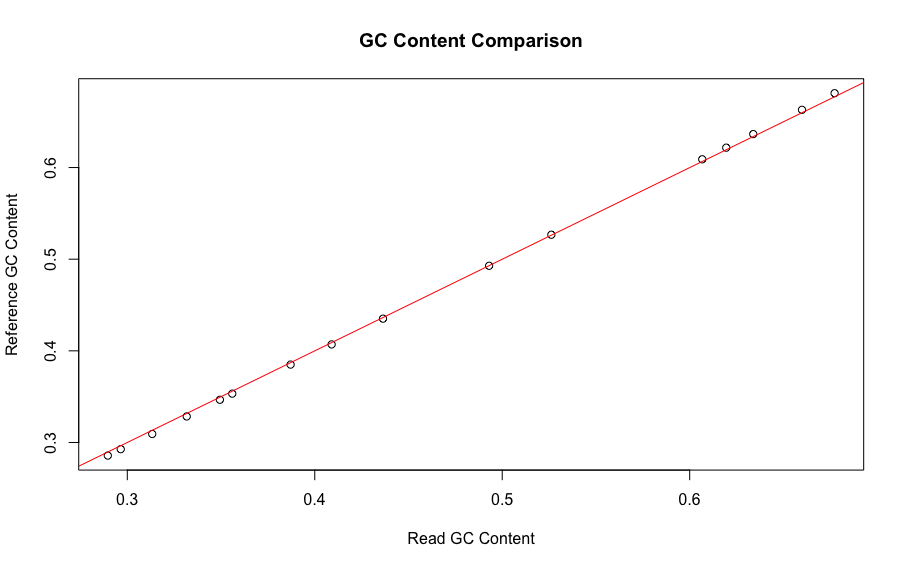
\includegraphics[height=4cm, width=6cm]{GC_Comparison.png} 
	\end{description}
	\end{frame}
	
	\begin{frame}{My Pipeline}
	\vspace{-1cm}
	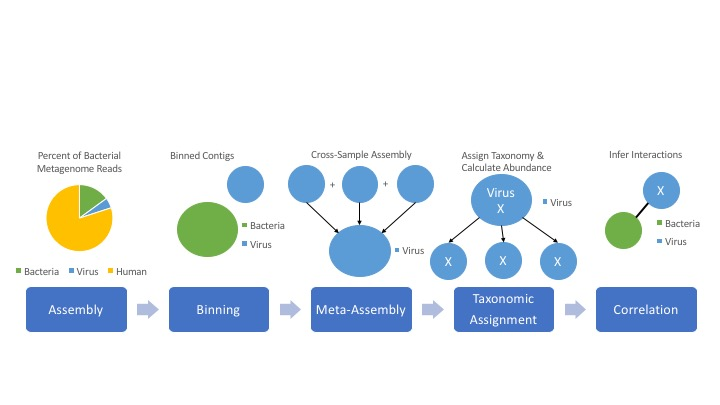
\includegraphics[height=6cm, width=11cm]{figure_2_updated.jpg}
	\end{frame}
	
	
	\begin{frame}{Performance Measurements}
	TP = True Positive; FP = False Positive; FN = False Negative
	\begin{block}{Precision}
	\begin{equation}
	P = \frac{TP} {TP + FP} \nonumber
	\end{equation}
	\end{block}
	\begin{block}{Recall}
	\begin{equation}
	R = \frac{TP}{TP + FN} \nonumber
	\end{equation}
	\end{block}
	\begin{block}{F1 Score}
	\begin{equation}
	F1 = \frac{2(TP)}{2(TP) + FP + FN} \nonumber
	\end{equation}
	\end{block}
	\end{frame}
	
	
	\begin{frame}{Results}
	Performance of methods identifying viral elements in simulated metagenome
	\begin{table}
	\begin{tabular}{|c || c | c | c | }
	\hline
	& \textbf{Precision} & \textbf{Recall} & \textbf{F1 Score} \\
	\hline
	\hline
	\textbf{Raw Reads} & 0.0593 & 1 & 0.1119 \\
	\hline
	\textbf{Full Assembly} & 0.3478 & 1 & 0.5161 \\
	\hline
	\textbf{Filter Pipeline} & \alert{0.4615} & 0.75 & \alert{0.5714} \\
	\hline
	\textbf{Blastx Filter} & 0.4444 & 0.5 & 0.4706 \\
	\hline
	\end{tabular}
	
	\caption{The F1 performance of the filter pipeline exceeds all other methods. The filtration method trades recall for overall performance.}
	\end{table}
	\end{frame}
	
	\begin{frame}{Troubleshooting}
	\begin{block}{Prophages}
	The bacterial genomes selected all contain prophage elements \\
	\tiny{Casjens, Sherwood. Molecular microbiology 2003}
	\end{block}
	\begin{block}{Prophage Discovery}
	The web-tool Phaster collected prophage prediction taxonomy on genomes used in simulation \\ \vspace{0.5cm} 
	No overlap of FP viruses and prophages predicted (Performed on Assembly and Filtered only)
	\end{block}
	\end{frame}
	
	

\section{BUD}
\subsection{}
	
	\begin{frame}{Data}
	A longitudinal survey of the Cystic Fibrosis airway of a single patient
	
	\begin{description}[Sequencing Data Information]
	\item[Number of Samples]	 36 Samples 
	\item[Avg Library Size] 33.3 Mb per Sample
	\item[Insert Size] 300 BPs non-paired (454 pyrosequencing)
	\item[Read Composition] Samples pre-filtered human samples using Deconseq \\
	\tiny{Schmieder, Robert, and Robert Edwards. PloS one 2011}
	\end{description}
	\end{frame}
	
	
	\begin{frame}{Synthetic Spike-In}
	To test sensitivity of pipeline added a rare virus to real dataset
	\begin{columns}
	\column{0.7\textwidth}
	\begin{block}{Zaire ebolavirus}
	18.96 Kb genome size \\ Generated 2000 reads using BBMap
	\end{block}
	
	\begin{block}{Synthetic Assembly}
	Generated a single contig 18.93Kb
	\end{block}
	
	\begin{block}{Distributed Reads}
	Incorporated 56 random ebola reads into samples
	\end{block}
	
	\column{0.35\textwidth}
	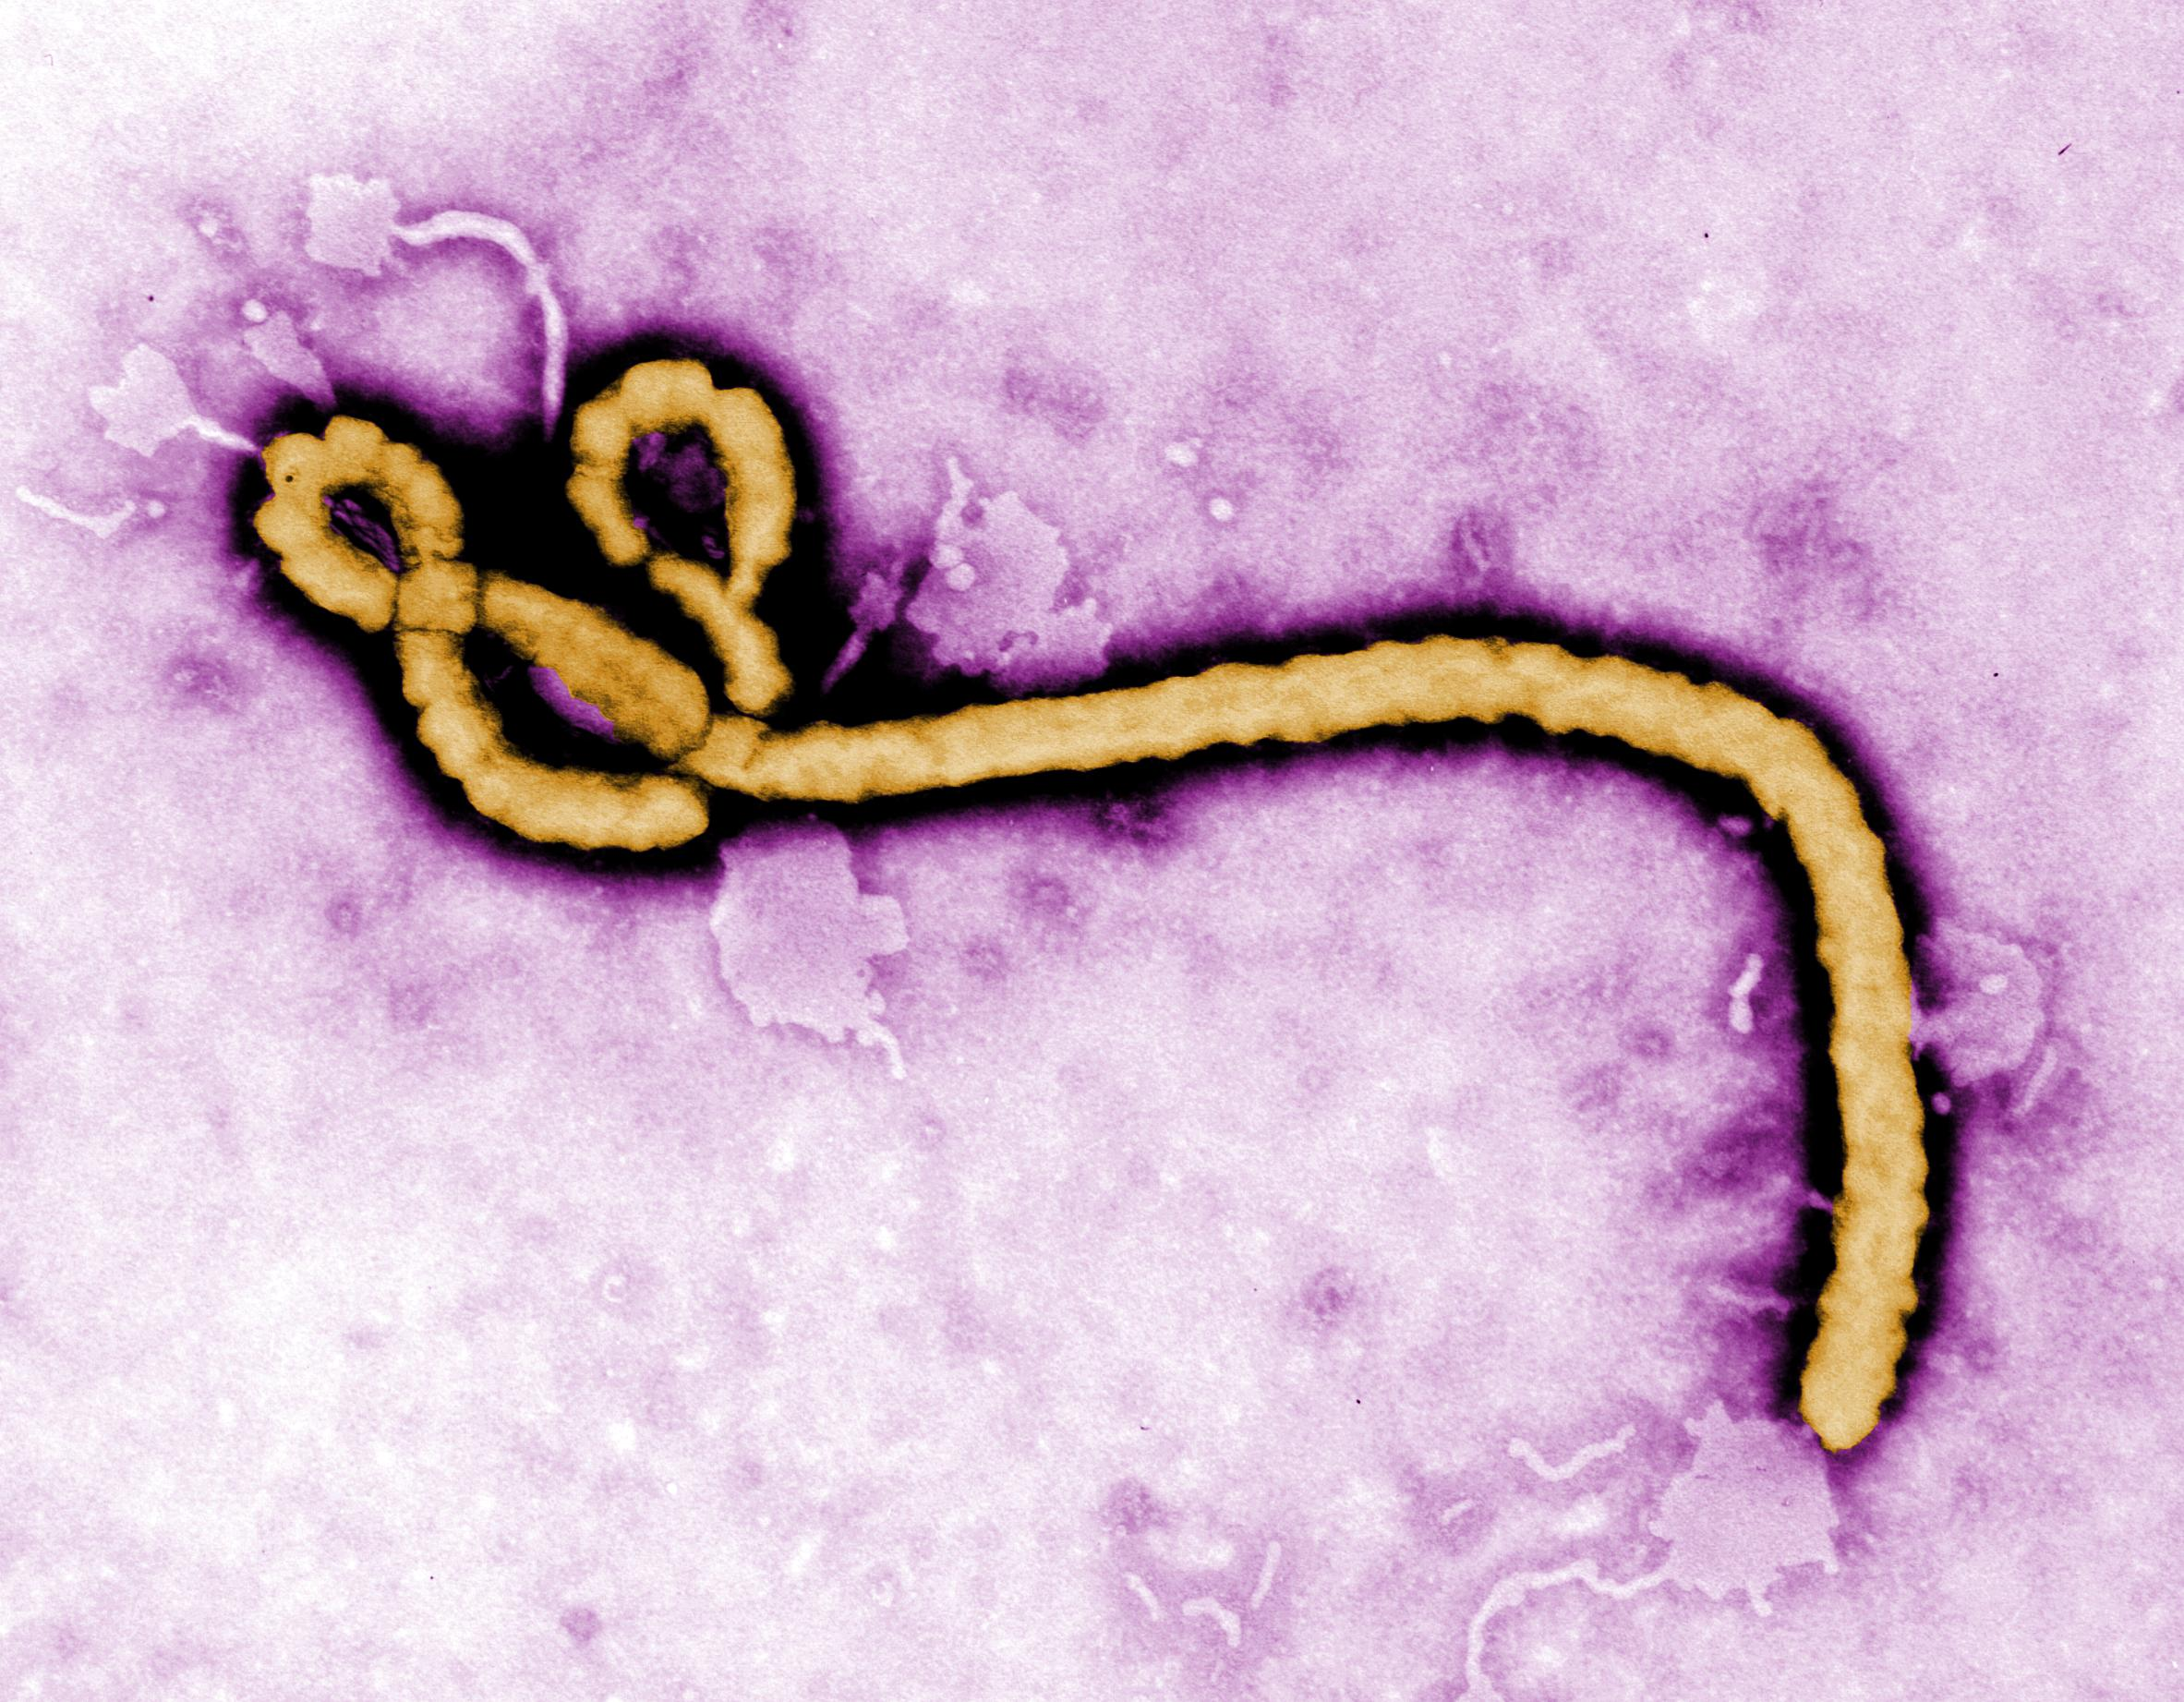
\includegraphics[height=3cm, width=3cm]{Ebola.jpg}
	\end{columns}
	\end{frame}
	
	\begin{frame}{Results}
	The results are based on presence absence in kraken taxonomic identities
	\begin{block}{Combined Sample Assembly}
	Identifies Zaire ebolavirus
	\end{block}
	
	\begin{block}{Significant Viral Contigs}
	Absent
	\end{block}
	
	\begin{block}{Viral Reads and Assembled}
	Absent
	\end{block}
	
	
	\end{frame}
	
	\begin{frame}{Discussion and Future Directions}
	
	\begin{block}{Synthetic Metagenome}
	\begin{itemize}
	\item The taxonomic identification performance of the filtration model exceeds that of both the raw and assembled reads. 
	\item Increasing the complexity of the simulation by both adding mutations and increasing the number of genomes is planned for this week. 
	\end{itemize}
	\end{block}
	\begin{block}{Synthetic Spike-In}
	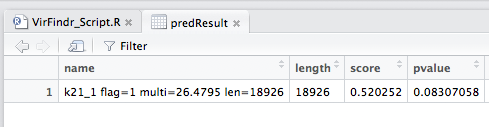
\includegraphics[height=2cm, width=8cm]{virfinder}
	\end{block}
	\end{frame}
	
\section{}
	
	\begin{frame}{}
	\vspace{1cm}
	{
\includegraphics[height=8cm, width=11cm]{Acknowledge.jpg} }
	\end{frame}
	
	
	\begin{frame}{Questions?}
	
	Cody Glickman \\ 
\includegraphics[height=2cm, width=2cm]{lablogo.png} \\ cody.glickman@ucdenver.edu \\ \alert{www.github.com/glickmac} \\ www.codyglickman.com
	\end{frame}
	
	
	\begin{frame}{Bias in Average Fold Coverage by GC}
	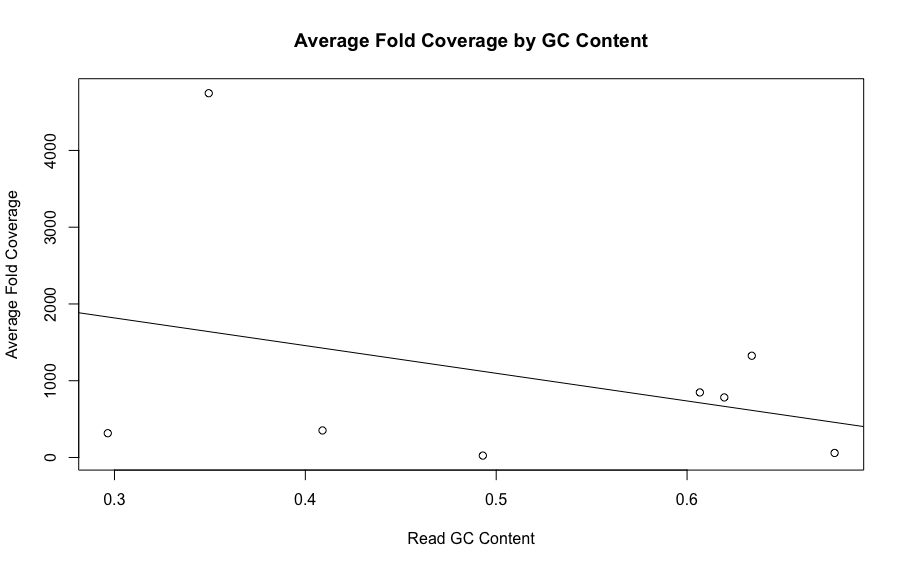
\includegraphics[height=8cm, width=11cm]{Viral_Coverage_by_GC.png}
	\end{frame}
	
	
	\begin{frame}{References}
	\tiny{ Barr, Jeremy, et al., PNAS 2013 \\ Tariq, Mohammad, et al., Frontiers in Microbiology 2015}
	\end{frame}
	
\end{document}